\documentclass[twoside]{book}

% Packages required by doxygen
\usepackage{calc}
\usepackage{doxygen}
\usepackage{graphicx}
\usepackage[utf8]{inputenc}
\usepackage{makeidx}
\usepackage{multicol}
\usepackage{multirow}
\usepackage{textcomp}
\usepackage[table]{xcolor}

% Font selection
\usepackage[T1]{fontenc}
\usepackage{mathptmx}
\usepackage[scaled=.90]{helvet}
\usepackage{courier}
\usepackage{amssymb}
\usepackage{sectsty}
\renewcommand{\familydefault}{\sfdefault}
\allsectionsfont{%
  \fontseries{bc}\selectfont%
  \color{darkgray}%
}
\renewcommand{\DoxyLabelFont}{%
  \fontseries{bc}\selectfont%
  \color{darkgray}%
}

% Page & text layout
\usepackage{geometry}
\geometry{%
  a4paper,%
  top=2.5cm,%
  bottom=2.5cm,%
  left=2.5cm,%
  right=2.5cm%
}
\tolerance=750
\hfuzz=15pt
\hbadness=750
\setlength{\emergencystretch}{15pt}
\setlength{\parindent}{0cm}
\setlength{\parskip}{0.2cm}
\makeatletter
\renewcommand{\paragraph}{%
  \@startsection{paragraph}{4}{0ex}{-1.0ex}{1.0ex}{%
    \normalfont\normalsize\bfseries\SS@parafont%
  }%
}
\renewcommand{\subparagraph}{%
  \@startsection{subparagraph}{5}{0ex}{-1.0ex}{1.0ex}{%
    \normalfont\normalsize\bfseries\SS@subparafont%
  }%
}
\makeatother

% Headers & footers
\usepackage{fancyhdr}
\pagestyle{fancyplain}
\fancyhead[LE]{\fancyplain{}{\bfseries\thepage}}
\fancyhead[CE]{\fancyplain{}{}}
\fancyhead[RE]{\fancyplain{}{\bfseries\leftmark}}
\fancyhead[LO]{\fancyplain{}{\bfseries\rightmark}}
\fancyhead[CO]{\fancyplain{}{}}
\fancyhead[RO]{\fancyplain{}{\bfseries\thepage}}
\fancyfoot[LE]{\fancyplain{}{}}
\fancyfoot[CE]{\fancyplain{}{}}
\fancyfoot[RE]{\fancyplain{}{\bfseries\scriptsize Generated on Wed Nov 18 2015 22\-:48\-:56 for My Project by Doxygen }}
\fancyfoot[LO]{\fancyplain{}{\bfseries\scriptsize Generated on Wed Nov 18 2015 22\-:48\-:56 for My Project by Doxygen }}
\fancyfoot[CO]{\fancyplain{}{}}
\fancyfoot[RO]{\fancyplain{}{}}
\renewcommand{\footrulewidth}{0.4pt}
\renewcommand{\chaptermark}[1]{%
  \markboth{#1}{}%
}
\renewcommand{\sectionmark}[1]{%
  \markright{\thesection\ #1}%
}

% Indices & bibliography
\usepackage{natbib}
\usepackage[titles]{tocloft}
\setcounter{tocdepth}{3}
\setcounter{secnumdepth}{5}
\makeindex

% Hyperlinks (required, but should be loaded last)
\usepackage{ifpdf}
\ifpdf
  \usepackage[pdftex,pagebackref=true]{hyperref}
\else
  \usepackage[ps2pdf,pagebackref=true]{hyperref}
\fi
\hypersetup{%
  colorlinks=true,%
  linkcolor=blue,%
  citecolor=blue,%
  unicode%
}

% Custom commands
\newcommand{\clearemptydoublepage}{%
  \newpage{\pagestyle{empty}\cleardoublepage}%
}


%===== C O N T E N T S =====

\begin{document}

% Titlepage & ToC
\hypersetup{pageanchor=false}
\pagenumbering{roman}
\begin{titlepage}
\vspace*{7cm}
\begin{center}%
{\Large My Project }\\
\vspace*{1cm}
{\large Generated by Doxygen 1.8.6}\\
\vspace*{0.5cm}
{\small Wed Nov 18 2015 22:48:56}\\
\end{center}
\end{titlepage}
\clearemptydoublepage
\tableofcontents
\clearemptydoublepage
\pagenumbering{arabic}
\hypersetup{pageanchor=true}

%--- Begin generated contents ---
\chapter{Hierarchical Index}
\section{Class Hierarchy}
This inheritance list is sorted roughly, but not completely, alphabetically\-:\begin{DoxyCompactList}
\item \contentsline{section}{Abstract\-Cell}{\pageref{classAbstractCell}}{}
\begin{DoxyCompactList}
\item \contentsline{section}{Conway\-Cell}{\pageref{classConwayCell}}{}
\item \contentsline{section}{Fredkin\-Cell}{\pageref{classFredkinCell}}{}
\end{DoxyCompactList}
\item \contentsline{section}{Cell}{\pageref{classCell}}{}
\item \contentsline{section}{Life$<$ C $>$}{\pageref{classLife}}{}
\end{DoxyCompactList}

\chapter{Class Index}
\section{Class List}
Here are the classes, structs, unions and interfaces with brief descriptions\-:\begin{DoxyCompactList}
\item\contentsline{section}{\hyperlink{classAbstractCell}{Abstract\-Cell} }{\pageref{classAbstractCell}}{}
\item\contentsline{section}{\hyperlink{classCell}{Cell} }{\pageref{classCell}}{}
\item\contentsline{section}{\hyperlink{classConwayCell}{Conway\-Cell} }{\pageref{classConwayCell}}{}
\item\contentsline{section}{\hyperlink{classFredkinCell}{Fredkin\-Cell} }{\pageref{classFredkinCell}}{}
\item\contentsline{section}{\hyperlink{classLife}{Life$<$ C $>$} }{\pageref{classLife}}{}
\end{DoxyCompactList}

\chapter{Class Documentation}
\hypertarget{classAbstractCell}{\section{Abstract\-Cell Class Reference}
\label{classAbstractCell}\index{Abstract\-Cell@{Abstract\-Cell}}
}
Inheritance diagram for Abstract\-Cell\-:\begin{figure}[H]
\begin{center}
\leavevmode
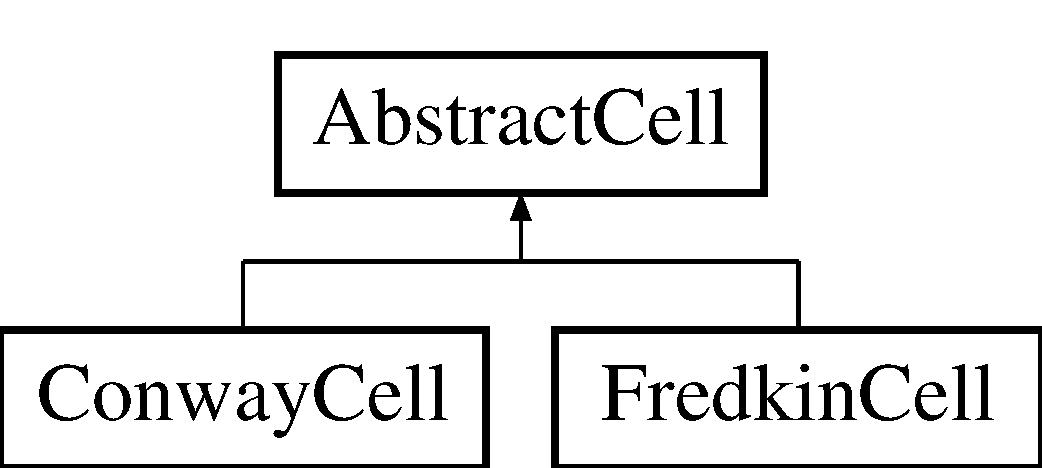
\includegraphics[height=2.000000cm]{classAbstractCell}
\end{center}
\end{figure}
\subsection*{Public Member Functions}
\begin{DoxyCompactItemize}
\item 
\hyperlink{classAbstractCell_a3f812bfb6db500d89323a4445bf2447f}{Abstract\-Cell} (char a)
\item 
virtual bool \hyperlink{classAbstractCell_ac2c599d61d1bafb09468b48204482f8b}{evolve} (\hyperlink{classAbstractCell}{Abstract\-Cell} $\ast$$\ast$const neighbors)=0
\item 
void \hyperlink{classAbstractCell_ae3d3e5b983c437cb77abffa49c8772e3}{shift\-\_\-state} ()
\item 
virtual char \hyperlink{classAbstractCell_a69ec6d128bfd858512fe6cb49676a03d}{state} ()=0
\item 
bool \hyperlink{classAbstractCell_aba811f858a0ec0c7e1d5f76960f78948}{living} ()
\end{DoxyCompactItemize}
\subsection*{Protected Attributes}
\begin{DoxyCompactItemize}
\item 
bool \hyperlink{classAbstractCell_aa92e42d5bb67f3249d8e2dde2c3228e7}{alive}
\end{DoxyCompactItemize}


\subsection{Constructor \& Destructor Documentation}
\hypertarget{classAbstractCell_a3f812bfb6db500d89323a4445bf2447f}{\index{Abstract\-Cell@{Abstract\-Cell}!Abstract\-Cell@{Abstract\-Cell}}
\index{Abstract\-Cell@{Abstract\-Cell}!AbstractCell@{Abstract\-Cell}}
\subsubsection[{Abstract\-Cell}]{\setlength{\rightskip}{0pt plus 5cm}Abstract\-Cell\-::\-Abstract\-Cell (
\begin{DoxyParamCaption}
\item[{char}]{a}
\end{DoxyParamCaption}
)}}\label{classAbstractCell_a3f812bfb6db500d89323a4445bf2447f}
Initialization of bool alive depends on char a. It's alive iff char a is not '-\/' or '.' 

\subsection{Member Function Documentation}
\hypertarget{classAbstractCell_ac2c599d61d1bafb09468b48204482f8b}{\index{Abstract\-Cell@{Abstract\-Cell}!evolve@{evolve}}
\index{evolve@{evolve}!AbstractCell@{Abstract\-Cell}}
\subsubsection[{evolve}]{\setlength{\rightskip}{0pt plus 5cm}virtual bool Abstract\-Cell\-::evolve (
\begin{DoxyParamCaption}
\item[{{\bf Abstract\-Cell} $\ast$$\ast$const}]{neighbors}
\end{DoxyParamCaption}
)\hspace{0.3cm}{\ttfamily [pure virtual]}}}\label{classAbstractCell_ac2c599d61d1bafb09468b48204482f8b}
Looks at the neighbors and return true iff bool alive needs to be changed. It's pure virtual so that child cells are forced to implement it. 

Implemented in \hyperlink{classFredkinCell_a0df0a7d13ac55700bfaf9d0d696e93ea}{Fredkin\-Cell}, and \hyperlink{classConwayCell_aa8221933ec26a3a3d92a53c89542da58}{Conway\-Cell}.

\hypertarget{classAbstractCell_aba811f858a0ec0c7e1d5f76960f78948}{\index{Abstract\-Cell@{Abstract\-Cell}!living@{living}}
\index{living@{living}!AbstractCell@{Abstract\-Cell}}
\subsubsection[{living}]{\setlength{\rightskip}{0pt plus 5cm}bool Abstract\-Cell\-::living (
\begin{DoxyParamCaption}
{}
\end{DoxyParamCaption}
)}}\label{classAbstractCell_aba811f858a0ec0c7e1d5f76960f78948}
Cells whether a cell is alive or not. Since that information is simply stored as a bool in state, I could just return the value of state. \hypertarget{classAbstractCell_ae3d3e5b983c437cb77abffa49c8772e3}{\index{Abstract\-Cell@{Abstract\-Cell}!shift\-\_\-state@{shift\-\_\-state}}
\index{shift\-\_\-state@{shift\-\_\-state}!AbstractCell@{Abstract\-Cell}}
\subsubsection[{shift\-\_\-state}]{\setlength{\rightskip}{0pt plus 5cm}void Abstract\-Cell\-::shift\-\_\-state (
\begin{DoxyParamCaption}
{}
\end{DoxyParamCaption}
)}}\label{classAbstractCell_ae3d3e5b983c437cb77abffa49c8772e3}
Shift the state of this cell. \hypertarget{classAbstractCell_a69ec6d128bfd858512fe6cb49676a03d}{\index{Abstract\-Cell@{Abstract\-Cell}!state@{state}}
\index{state@{state}!AbstractCell@{Abstract\-Cell}}
\subsubsection[{state}]{\setlength{\rightskip}{0pt plus 5cm}virtual char Abstract\-Cell\-::state (
\begin{DoxyParamCaption}
{}
\end{DoxyParamCaption}
)\hspace{0.3cm}{\ttfamily [pure virtual]}}}\label{classAbstractCell_a69ec6d128bfd858512fe6cb49676a03d}
Return a char representing the current state for the corresponding class. Since the two cells have different representative characters, this is abstract 

Implemented in \hyperlink{classFredkinCell_a52dae5bfba89995f7cf6a1881de0b4cf}{Fredkin\-Cell}, and \hyperlink{classConwayCell_ab5b50f8f1e4898961e53c0f88c52e804}{Conway\-Cell}.



\subsection{Member Data Documentation}
\hypertarget{classAbstractCell_aa92e42d5bb67f3249d8e2dde2c3228e7}{\index{Abstract\-Cell@{Abstract\-Cell}!alive@{alive}}
\index{alive@{alive}!AbstractCell@{Abstract\-Cell}}
\subsubsection[{alive}]{\setlength{\rightskip}{0pt plus 5cm}bool Abstract\-Cell\-::alive\hspace{0.3cm}{\ttfamily [protected]}}}\label{classAbstractCell_aa92e42d5bb67f3249d8e2dde2c3228e7}
Stores cell's life status 

The documentation for this class was generated from the following files\-:\begin{DoxyCompactItemize}
\item 
Life.\-h\item 
Life.\-c++\end{DoxyCompactItemize}

\hypertarget{classCell}{\section{Cell Class Reference}
\label{classCell}\index{Cell@{Cell}}
}
\subsection*{Public Member Functions}
\begin{DoxyCompactItemize}
\item 
\hyperlink{classCell_a297c04746ff5d676b6814c66d4a7cd5f}{Cell} (char a)
\item 
\hyperlink{classCell_a93fb42df05d8c92468799093c527e5f1}{Cell} (const \hyperlink{classCell}{Cell} \&rhs)
\item 
\hyperlink{classCell_a9fa559f7a28e2b4336c6879ca09304d8}{$\sim$\-Cell} ()
\item 
bool \hyperlink{classCell_a8f5886fbfafc044567b320b30f5b7cfa}{evolve} (\hyperlink{classAbstractCell}{Abstract\-Cell} $\ast$$\ast$const neighbors)
\item 
\hyperlink{classAbstractCell}{Abstract\-Cell} $\ast$ \hyperlink{classCell_adacf5a139b7a3521ec8bec7817476997}{operator\&} ()
\item 
void \hyperlink{classCell_a04ea1962372996c88fd00e6bc2fb815d}{shift\-\_\-state} ()
\item 
char \hyperlink{classCell_a5ef815a51cac8abe3280c986aa95e5f7}{state} ()
\item 
bool \hyperlink{classCell_aa2694791e33edaa1f9cbc2c0d7897b92}{living} ()
\end{DoxyCompactItemize}


\subsection{Constructor \& Destructor Documentation}
\hypertarget{classCell_a297c04746ff5d676b6814c66d4a7cd5f}{\index{Cell@{Cell}!Cell@{Cell}}
\index{Cell@{Cell}!Cell@{Cell}}
\subsubsection[{Cell}]{\setlength{\rightskip}{0pt plus 5cm}Cell\-::\-Cell (
\begin{DoxyParamCaption}
\item[{char}]{a}
\end{DoxyParamCaption}
)}}\label{classCell_a297c04746ff5d676b6814c66d4a7cd5f}
Makes a new Conway\-Cell/\-Fredkin\-Cell for \-\_\-p. \hypertarget{classCell_a93fb42df05d8c92468799093c527e5f1}{\index{Cell@{Cell}!Cell@{Cell}}
\index{Cell@{Cell}!Cell@{Cell}}
\subsubsection[{Cell}]{\setlength{\rightskip}{0pt plus 5cm}Cell\-::\-Cell (
\begin{DoxyParamCaption}
\item[{const {\bf Cell} \&}]{rhs}
\end{DoxyParamCaption}
)}}\label{classCell_a93fb42df05d8c92468799093c527e5f1}
Copies the \hyperlink{classAbstractCell}{Abstract\-Cell} present into \-\_\-p \hypertarget{classCell_a9fa559f7a28e2b4336c6879ca09304d8}{\index{Cell@{Cell}!$\sim$\-Cell@{$\sim$\-Cell}}
\index{$\sim$\-Cell@{$\sim$\-Cell}!Cell@{Cell}}
\subsubsection[{$\sim$\-Cell}]{\setlength{\rightskip}{0pt plus 5cm}Cell\-::$\sim$\-Cell (
\begin{DoxyParamCaption}
{}
\end{DoxyParamCaption}
)}}\label{classCell_a9fa559f7a28e2b4336c6879ca09304d8}
Deallocates \-\_\-p space. 

\subsection{Member Function Documentation}
\hypertarget{classCell_a8f5886fbfafc044567b320b30f5b7cfa}{\index{Cell@{Cell}!evolve@{evolve}}
\index{evolve@{evolve}!Cell@{Cell}}
\subsubsection[{evolve}]{\setlength{\rightskip}{0pt plus 5cm}bool Cell\-::evolve (
\begin{DoxyParamCaption}
\item[{{\bf Abstract\-Cell} $\ast$$\ast$const}]{neighbors}
\end{DoxyParamCaption}
)}}\label{classCell_a8f5886fbfafc044567b320b30f5b7cfa}
Run's the cell's evolve, and changes the \hyperlink{classFredkinCell}{Fredkin\-Cell} if needed \hypertarget{classCell_aa2694791e33edaa1f9cbc2c0d7897b92}{\index{Cell@{Cell}!living@{living}}
\index{living@{living}!Cell@{Cell}}
\subsubsection[{living}]{\setlength{\rightskip}{0pt plus 5cm}bool Cell\-::living (
\begin{DoxyParamCaption}
{}
\end{DoxyParamCaption}
)}}\label{classCell_aa2694791e33edaa1f9cbc2c0d7897b92}
Runs \hyperlink{classCell_aa2694791e33edaa1f9cbc2c0d7897b92}{living()} for the cell type \hypertarget{classCell_adacf5a139b7a3521ec8bec7817476997}{\index{Cell@{Cell}!operator\&@{operator\&}}
\index{operator\&@{operator\&}!Cell@{Cell}}
\subsubsection[{operator\&}]{\setlength{\rightskip}{0pt plus 5cm}{\bf Abstract\-Cell} $\ast$ Cell\-::operator\& (
\begin{DoxyParamCaption}
{}
\end{DoxyParamCaption}
)}}\label{classCell_adacf5a139b7a3521ec8bec7817476997}
Overloaded operator\& to return \-\_\-p \hypertarget{classCell_a04ea1962372996c88fd00e6bc2fb815d}{\index{Cell@{Cell}!shift\-\_\-state@{shift\-\_\-state}}
\index{shift\-\_\-state@{shift\-\_\-state}!Cell@{Cell}}
\subsubsection[{shift\-\_\-state}]{\setlength{\rightskip}{0pt plus 5cm}void Cell\-::shift\-\_\-state (
\begin{DoxyParamCaption}
{}
\end{DoxyParamCaption}
)}}\label{classCell_a04ea1962372996c88fd00e6bc2fb815d}
Runs \hyperlink{classCell_a04ea1962372996c88fd00e6bc2fb815d}{shift\-\_\-state()} for the cell type \hypertarget{classCell_a5ef815a51cac8abe3280c986aa95e5f7}{\index{Cell@{Cell}!state@{state}}
\index{state@{state}!Cell@{Cell}}
\subsubsection[{state}]{\setlength{\rightskip}{0pt plus 5cm}char Cell\-::state (
\begin{DoxyParamCaption}
{}
\end{DoxyParamCaption}
)}}\label{classCell_a5ef815a51cac8abe3280c986aa95e5f7}
Runs \hyperlink{classCell_a5ef815a51cac8abe3280c986aa95e5f7}{state()} for the cell type 

The documentation for this class was generated from the following files\-:\begin{DoxyCompactItemize}
\item 
Life.\-h\item 
Life.\-c++\end{DoxyCompactItemize}

\hypertarget{classConwayCell}{\section{Conway\-Cell Class Reference}
\label{classConwayCell}\index{Conway\-Cell@{Conway\-Cell}}
}
Inheritance diagram for Conway\-Cell\-:\begin{figure}[H]
\begin{center}
\leavevmode
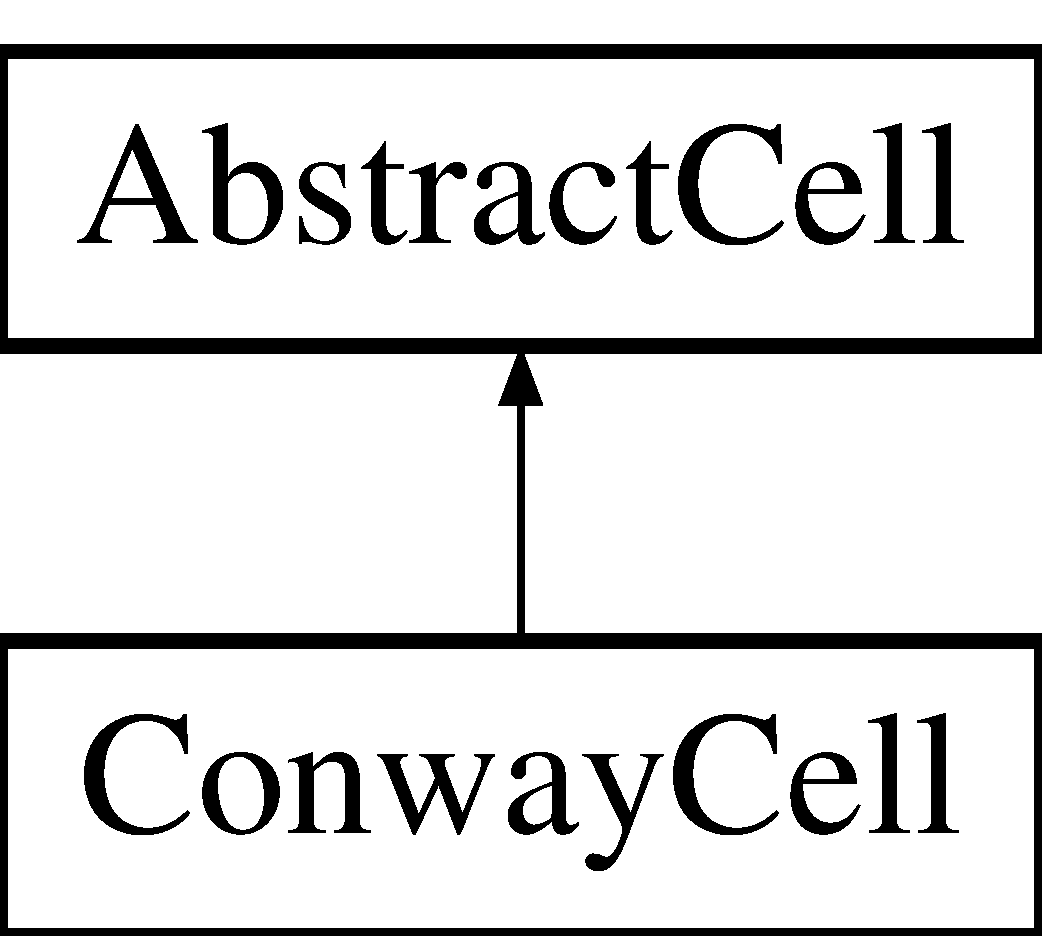
\includegraphics[height=2.000000cm]{classConwayCell}
\end{center}
\end{figure}
\subsection*{Public Member Functions}
\begin{DoxyCompactItemize}
\item 
\hyperlink{classConwayCell_a2958b6bb4801d59156d3640d57cd0225}{Conway\-Cell} (char a)
\item 
bool \hyperlink{classConwayCell_aa8221933ec26a3a3d92a53c89542da58}{evolve} (\hyperlink{classAbstractCell}{Abstract\-Cell} $\ast$$\ast$const n)
\item 
char \hyperlink{classConwayCell_ab5b50f8f1e4898961e53c0f88c52e804}{state} ()
\end{DoxyCompactItemize}
\subsection*{Additional Inherited Members}


\subsection{Constructor \& Destructor Documentation}
\hypertarget{classConwayCell_a2958b6bb4801d59156d3640d57cd0225}{\index{Conway\-Cell@{Conway\-Cell}!Conway\-Cell@{Conway\-Cell}}
\index{Conway\-Cell@{Conway\-Cell}!ConwayCell@{Conway\-Cell}}
\subsubsection[{Conway\-Cell}]{\setlength{\rightskip}{0pt plus 5cm}Conway\-Cell\-::\-Conway\-Cell (
\begin{DoxyParamCaption}
\item[{char}]{a}
\end{DoxyParamCaption}
)}}\label{classConwayCell_a2958b6bb4801d59156d3640d57cd0225}
Constructs a Conway cell with the argument 

\subsection{Member Function Documentation}
\hypertarget{classConwayCell_aa8221933ec26a3a3d92a53c89542da58}{\index{Conway\-Cell@{Conway\-Cell}!evolve@{evolve}}
\index{evolve@{evolve}!ConwayCell@{Conway\-Cell}}
\subsubsection[{evolve}]{\setlength{\rightskip}{0pt plus 5cm}bool Conway\-Cell\-::evolve (
\begin{DoxyParamCaption}
\item[{{\bf Abstract\-Cell} $\ast$$\ast$const}]{n}
\end{DoxyParamCaption}
)\hspace{0.3cm}{\ttfamily [virtual]}}}\label{classConwayCell_aa8221933ec26a3a3d92a53c89542da58}
Returns true if the state needs to be changed. n is for neighbors 

Implements \hyperlink{classAbstractCell_ac2c599d61d1bafb09468b48204482f8b}{Abstract\-Cell}.

\hypertarget{classConwayCell_ab5b50f8f1e4898961e53c0f88c52e804}{\index{Conway\-Cell@{Conway\-Cell}!state@{state}}
\index{state@{state}!ConwayCell@{Conway\-Cell}}
\subsubsection[{state}]{\setlength{\rightskip}{0pt plus 5cm}char Conway\-Cell\-::state (
\begin{DoxyParamCaption}
{}
\end{DoxyParamCaption}
)\hspace{0.3cm}{\ttfamily [virtual]}}}\label{classConwayCell_ab5b50f8f1e4898961e53c0f88c52e804}
Prints the symbol of the state. '$\ast$' for alive, else '.' 

Implements \hyperlink{classAbstractCell_a69ec6d128bfd858512fe6cb49676a03d}{Abstract\-Cell}.



The documentation for this class was generated from the following files\-:\begin{DoxyCompactItemize}
\item 
Life.\-h\item 
Life.\-c++\end{DoxyCompactItemize}

\hypertarget{classFredkinCell}{\section{Fredkin\-Cell Class Reference}
\label{classFredkinCell}\index{Fredkin\-Cell@{Fredkin\-Cell}}
}
Inheritance diagram for Fredkin\-Cell\-:\begin{figure}[H]
\begin{center}
\leavevmode
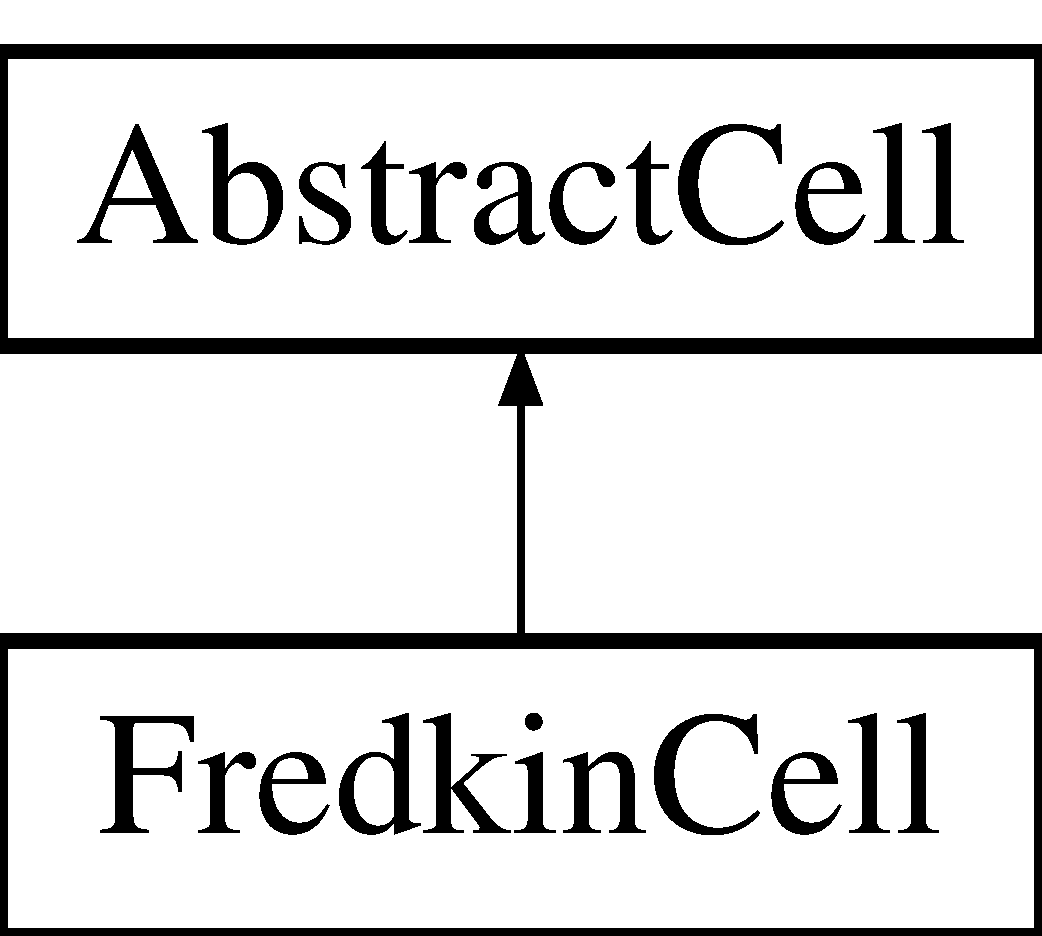
\includegraphics[height=2.000000cm]{classFredkinCell}
\end{center}
\end{figure}
\subsection*{Public Member Functions}
\begin{DoxyCompactItemize}
\item 
\hyperlink{classFredkinCell_a45b59868c0c390a05b8555df2c197136}{Fredkin\-Cell} (char a)
\item 
bool \hyperlink{classFredkinCell_a0df0a7d13ac55700bfaf9d0d696e93ea}{evolve} (\hyperlink{classAbstractCell}{Abstract\-Cell} $\ast$$\ast$const n)
\item 
char \hyperlink{classFredkinCell_a52dae5bfba89995f7cf6a1881de0b4cf}{state} ()
\end{DoxyCompactItemize}
\subsection*{Additional Inherited Members}


\subsection{Constructor \& Destructor Documentation}
\hypertarget{classFredkinCell_a45b59868c0c390a05b8555df2c197136}{\index{Fredkin\-Cell@{Fredkin\-Cell}!Fredkin\-Cell@{Fredkin\-Cell}}
\index{Fredkin\-Cell@{Fredkin\-Cell}!FredkinCell@{Fredkin\-Cell}}
\subsubsection[{Fredkin\-Cell}]{\setlength{\rightskip}{0pt plus 5cm}Fredkin\-Cell\-::\-Fredkin\-Cell (
\begin{DoxyParamCaption}
\item[{char}]{a}
\end{DoxyParamCaption}
)}}\label{classFredkinCell_a45b59868c0c390a05b8555df2c197136}
Initializes age based on char a 

\subsection{Member Function Documentation}
\hypertarget{classFredkinCell_a0df0a7d13ac55700bfaf9d0d696e93ea}{\index{Fredkin\-Cell@{Fredkin\-Cell}!evolve@{evolve}}
\index{evolve@{evolve}!FredkinCell@{Fredkin\-Cell}}
\subsubsection[{evolve}]{\setlength{\rightskip}{0pt plus 5cm}bool Fredkin\-Cell\-::evolve (
\begin{DoxyParamCaption}
\item[{{\bf Abstract\-Cell} $\ast$$\ast$const}]{n}
\end{DoxyParamCaption}
)\hspace{0.3cm}{\ttfamily [virtual]}}}\label{classFredkinCell_a0df0a7d13ac55700bfaf9d0d696e93ea}
Returns true if the state needs to be changed. n is for neighbors Needs to change it's age as well as state 

Implements \hyperlink{classAbstractCell_ac2c599d61d1bafb09468b48204482f8b}{Abstract\-Cell}.

\hypertarget{classFredkinCell_a52dae5bfba89995f7cf6a1881de0b4cf}{\index{Fredkin\-Cell@{Fredkin\-Cell}!state@{state}}
\index{state@{state}!FredkinCell@{Fredkin\-Cell}}
\subsubsection[{state}]{\setlength{\rightskip}{0pt plus 5cm}char Fredkin\-Cell\-::state (
\begin{DoxyParamCaption}
{}
\end{DoxyParamCaption}
)\hspace{0.3cm}{\ttfamily [virtual]}}}\label{classFredkinCell_a52dae5bfba89995f7cf6a1881de0b4cf}
Prints the symbol of the state. An int for alive, else '-\/' 

Implements \hyperlink{classAbstractCell_a69ec6d128bfd858512fe6cb49676a03d}{Abstract\-Cell}.



The documentation for this class was generated from the following files\-:\begin{DoxyCompactItemize}
\item 
Life.\-h\item 
Life.\-c++\end{DoxyCompactItemize}

\hypertarget{classLife}{\section{Life$<$ C $>$ Class Template Reference}
\label{classLife}\index{Life$<$ C $>$@{Life$<$ C $>$}}
}
\subsection*{Public Member Functions}
\begin{DoxyCompactItemize}
\item 
\hyperlink{classLife_a9cbcf23c08a0e3e62c4094a7f67fb52c}{Life} (istream \&in)
\item 
void \hyperlink{classLife_a3b01c2be2fe838b5ee92cb14d5c27a69}{print\-\_\-grid} (int g, ostream \&w)
\item 
C \& \hyperlink{classLife_a27f2747e2acad26417888d9930556fd0}{at} (int n)
\item 
\hypertarget{classLife_a791fd29a0c0a0d958f5de0b46612af0f}{C $\ast$ {\bfseries begin} ()}\label{classLife_a791fd29a0c0a0d958f5de0b46612af0f}

\item 
\hypertarget{classLife_ab1468dd9d0805d05f97cde7b4952430e}{C $\ast$ {\bfseries end} ()}\label{classLife_ab1468dd9d0805d05f97cde7b4952430e}

\end{DoxyCompactItemize}
\subsection*{Public Attributes}
\begin{DoxyCompactItemize}
\item 
int \hyperlink{classLife_ad22f68d858f4b7499a80787bf22db860}{e}
\item 
\hypertarget{classLife_aa71fab541a96ce7ae6653249d09fc663}{int {\bfseries f}}\label{classLife_aa71fab541a96ce7ae6653249d09fc663}

\end{DoxyCompactItemize}


\subsection{Constructor \& Destructor Documentation}
\hypertarget{classLife_a9cbcf23c08a0e3e62c4094a7f67fb52c}{\index{Life@{Life}!Life@{Life}}
\index{Life@{Life}!Life@{Life}}
\subsubsection[{Life}]{\setlength{\rightskip}{0pt plus 5cm}template$<$typename C $>$ {\bf Life}$<$ C $>$\-::{\bf Life} (
\begin{DoxyParamCaption}
\item[{istream \&}]{in}
\end{DoxyParamCaption}
)\hspace{0.3cm}{\ttfamily [inline]}}}\label{classLife_a9cbcf23c08a0e3e62c4094a7f67fb52c}
Makes a grid based on the received input. 

\subsection{Member Function Documentation}
\hypertarget{classLife_a27f2747e2acad26417888d9930556fd0}{\index{Life@{Life}!at@{at}}
\index{at@{at}!Life@{Life}}
\subsubsection[{at}]{\setlength{\rightskip}{0pt plus 5cm}template$<$typename C $>$ C\& {\bf Life}$<$ C $>$\-::at (
\begin{DoxyParamCaption}
\item[{int}]{n}
\end{DoxyParamCaption}
)\hspace{0.3cm}{\ttfamily [inline]}}}\label{classLife_a27f2747e2acad26417888d9930556fd0}
Make the grid in \hyperlink{classLife}{Life} iterable \hypertarget{classLife_a3b01c2be2fe838b5ee92cb14d5c27a69}{\index{Life@{Life}!print\-\_\-grid@{print\-\_\-grid}}
\index{print\-\_\-grid@{print\-\_\-grid}!Life@{Life}}
\subsubsection[{print\-\_\-grid}]{\setlength{\rightskip}{0pt plus 5cm}template$<$typename C $>$ void {\bf Life}$<$ C $>$\-::print\-\_\-grid (
\begin{DoxyParamCaption}
\item[{int}]{g, }
\item[{ostream \&}]{w}
\end{DoxyParamCaption}
)\hspace{0.3cm}{\ttfamily [inline]}}}\label{classLife_a3b01c2be2fe838b5ee92cb14d5c27a69}
Prints the grid of the current generation, g. 

\subsection{Member Data Documentation}
\hypertarget{classLife_ad22f68d858f4b7499a80787bf22db860}{\index{Life@{Life}!e@{e}}
\index{e@{e}!Life@{Life}}
\subsubsection[{e}]{\setlength{\rightskip}{0pt plus 5cm}template$<$typename C $>$ int {\bf Life}$<$ C $>$\-::e}}\label{classLife_ad22f68d858f4b7499a80787bf22db860}
These save the number of evolutions and frequency of prints 

The documentation for this class was generated from the following file\-:\begin{DoxyCompactItemize}
\item 
Life.\-h\end{DoxyCompactItemize}

%--- End generated contents ---

% Index
\newpage
\phantomsection
\addcontentsline{toc}{chapter}{Index}
\printindex

\end{document}
